\chapter{蓝海枢纽系统架构与关键技术体系}

本章回答“系统由什么组成、模块怎样连接、哪些技术尚需验证”。设备工作原理、物理接口、
控制责任和TRL证据在本章集中管理；参数进入第4章后不再重复设备案例，仿真性能进入
第5章后不回写为设备固有性能，投资与政策含义由第6章承接。

\begin{figure}[H]
\centering
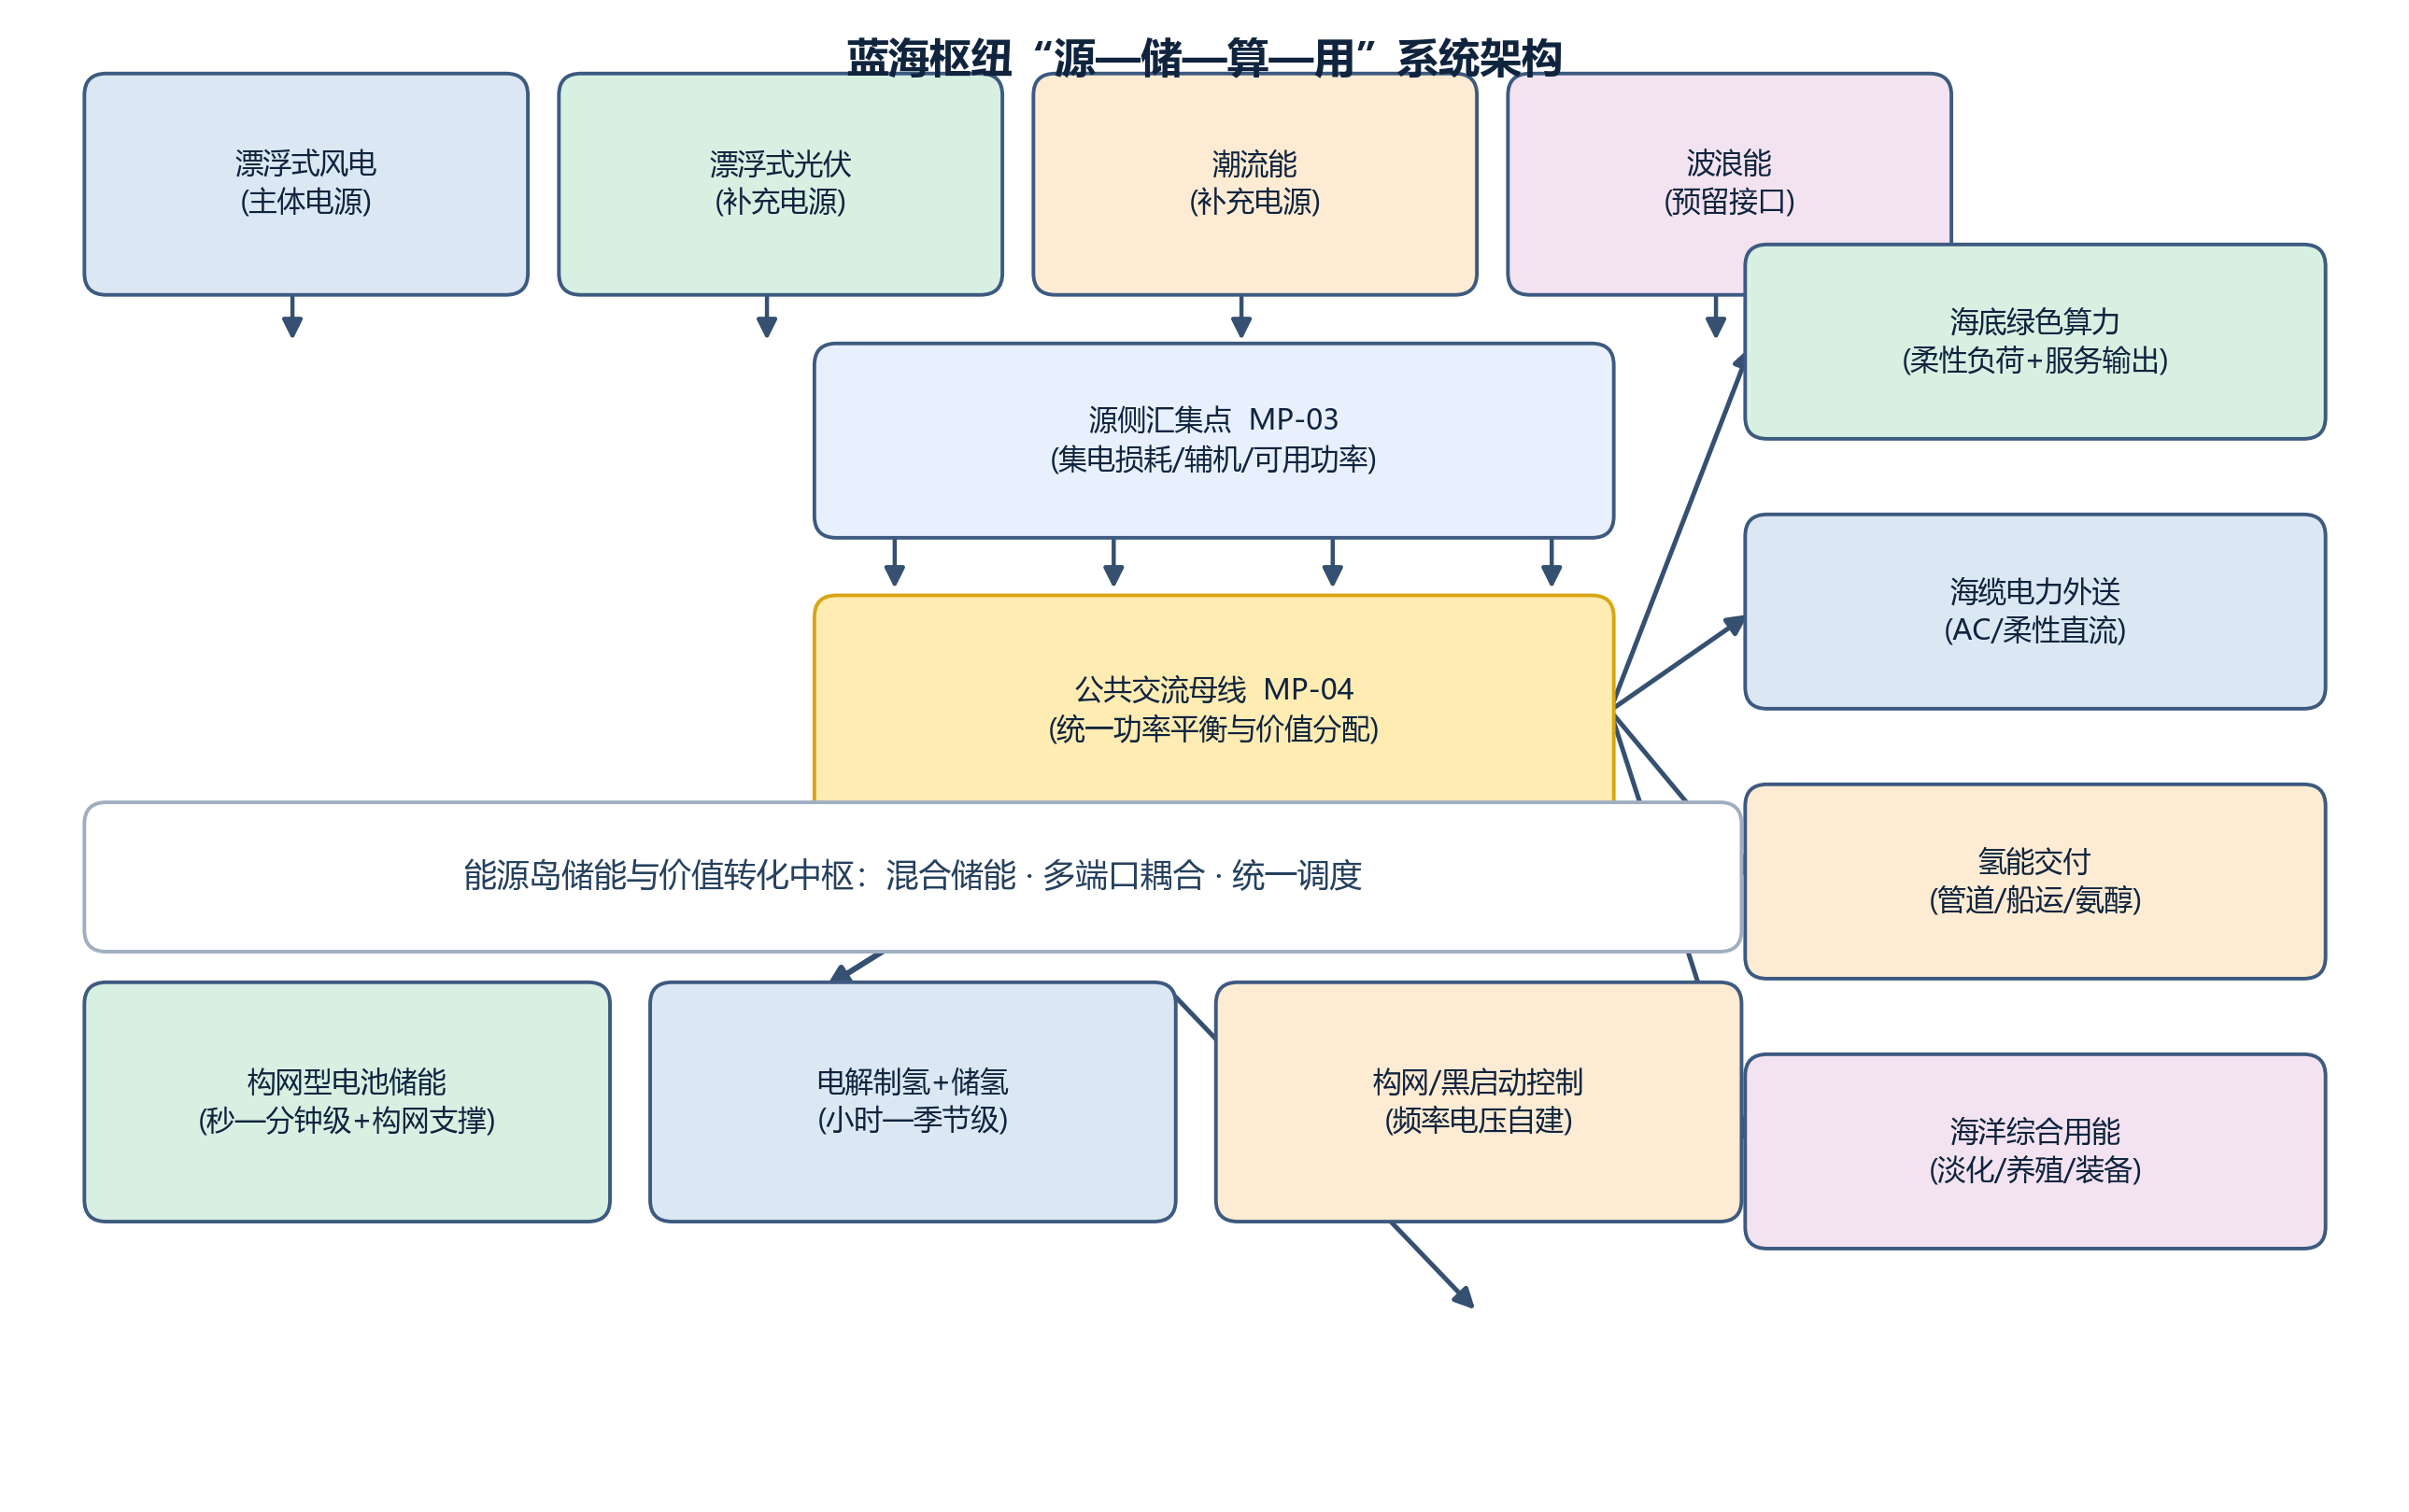
\includegraphics[width=0.98\textwidth]{figures/chapter3/fig3-1_system_architecture.png}
\caption{蓝海枢纽“源—储—算—用”总体功能架构}
\label{fig:c3-architecture}
\sourcetype{项目内部系统架构图。图中模块容量及占比不构成工程定值。}
\end{figure}

总体架构由五个层次组成：多源供给层产生逐时可用功率；公共母线与构网单元建立电压、
频率和功率平衡基准；电池、制氢储氢和柔性算力跨时间尺度调节；外送端口完成电力、氢能、
算力和海洋服务交付；协同调度大脑在设备安全控制之上执行预测、滚动优化、计量和结算。

\section{多源能源供给层}

\subsection{电源层级与容量边界}

多源供给采用“主体电源—互补电源—预留电源”三级结构。漂浮式风电承担主体供能，
漂浮式光伏用于日内互补，波浪能和潮流能作为标准化接口及情景选项。项目提出风电容量
占比不低于85\%\assumptiontag；该比例只表示架构方向，不作为模型结果，最终配置由
场址资源、平台载荷、设备曲线和第4、5章容量—运行联合分析确定。

\begin{table}[H]
\centering
\caption{多源供给模块的功能边界与模型接口}
\label{tab:c3-source-boundary}
\begin{tabularx}{\textwidth}{p{2.5cm} p{2.5cm} X X}
\toprule
模块 & 架构角色 & 第3章冻结的工程边界 & 交给第4章的输入\\
\midrule
漂浮式风电 & 主体电源 & 风机—浮体—系泊—动态电缆耦合；切入、额定、切出与复归状态 & 场址风速、厂家功率曲线、可用率和限发状态\\
漂浮式光伏 & 日间互补 & 组件温度、倾角、波致运动、盐雾与清洗；平台面积和载荷 & 辐照、温度、功率矩阵、可用面积和辅机功率\\
潮流能 & 可预测补充/预留 & 涨落潮双向特性、换向区和停机边界 & 流速序列、双向功率曲线、状态标识\\
波浪能 & 资源补充/预留 & 波高—周期二维功率矩阵及生存工况 & 海况联合分布、功率矩阵、停机与复归状态\\
源侧辅机 & 刚性负荷 & 泵、控制、通信、加热、除湿等不得隐藏在净发电量中 & 分项辅机负荷与启停逻辑\\
\bottomrule
\end{tabularx}
\sourcetype{项目内部架构；功率曲线和环境边界须来自设备商、型式试验、国际/行业标准或企业访谈一手数据。}
\end{table}

本项目不把发电量预先“定死”。每个时段的可用功率由资源序列、设备功率曲线、容量、
可用状态和环境限制共同产生；只有达到额定容量或安全限值时才截断。第4章给出数学表达，
第5章据仿真输出统计发电量和弃能量。

\subsection{互补性与不确定性处理}

风、光、浪、流可能在部分时段互补，也可能在持续低风、阴雨或设备避险时共同不足。
因此，互补性不能用静态容量比例宣告，而应通过同一时间轴上的资源数据检验。设计阶段
至少保留三类信息：逐时预测值、预测误差区间和设备可用状态；调度层只使用决策时点已
获得的数据，真实出力在下一时段到达后更新。

第3章不再保留原稿中“多源叠加后波动系数下降至某数值”等模型结果。平滑效果、弃能
变化和容量因子属于第5章输出，需分别在正常典型48 h、完整年度和极端事件中统计。

\subsection{海洋环境、台风与恢复状态}

漂浮式风机的场址外部条件、设计载荷工况、浮体控制和安全完整性应依据IEC 61400-3-2
及适用的国内标准开展工程设计\cite{iec61400-3-2,gbz44047}。标准能够定义评估框架，
不能替代目标海域测风测海、地质勘察和厂家载荷包。
\sourcetype{国际标准、国家标准化指导性技术文件。}

为使极端事件能够进入第5章，所有海上电源统一设置四类状态：
\begin{enumerate}
  \item {\bfseries 正常运行：}资源和设备均在连续运行边界内；
  \item {\bfseries 受限运行：}降载、限功率或部分模块停运，仍可接受调度指令；
  \item {\bfseries 生存停机：}台风、极端浪流或故障触发保护，出力不可由经济优化恢复；
  \item {\bfseries 检查复归：}事件后按检查、通信确认、辅机恢复和分级并网顺序返回运行。
\end{enumerate}

触发阈值、提前避险时间和复归时长均为设备与场址专属数据，若无OEM和海试证据应标注
为\assumptiontag。年度仿真必须显式包含极端事件及恢复期，不能只在正常曲线中降低
平均可用率。

\subsection{源侧物理、数据与控制接口}

\begin{table}[H]
\centering
\caption{源侧接口最小集合}
\label{tab:c3-source-interface}
\begin{tabularx}{\textwidth}{p{2.5cm} X X}
\toprule
接口类型 & 上送调度平台 & 调度平台下发\\
\midrule
物理接口 & 端口有功/无功、母线电压、电流、断路器状态 & 有功限值、无功/电压目标、启停许可\\
资源接口 & 风速风向、辐照温度、波高周期、流速流向 & 预测版本号、可信区间和更新周期\\
设备接口 & 可用容量、告警、降额原因、检修窗口、复归条件 & 运行模式、功率爬坡、检修协调\\
安全接口 & 极端天气级别、结构/系泊/海缆监测、保护动作 & 避险指令、孤岛切换、应急停机\\
计量接口 & 毛发电、辅机耗电、净注入、弃能原因 & 计量校验、时间同步和数据质量标识\\
\bottomrule
\end{tabularx}
\sourcetype{项目内部接口定义；最终字段须由OEM、设计院、调度及通信单位联合冻结。}
\end{table}

\section{构网型混合储能与价值转化中枢}

\subsection{多时间尺度责任分工}

混合储能的价值来自责任分层，而不是把所有储能等效为一个能量池。构网型电池承担
毫秒至小时范围内的基准建立、快速功率支撑和短时能量搬移；电解槽、储氢和产品库存
承担小时至更长时间尺度的柔性吸纳与价值转换。二者在公共母线相遇，但控制器、约束和
验收方法不同。

\begin{figure}[H]
\centering
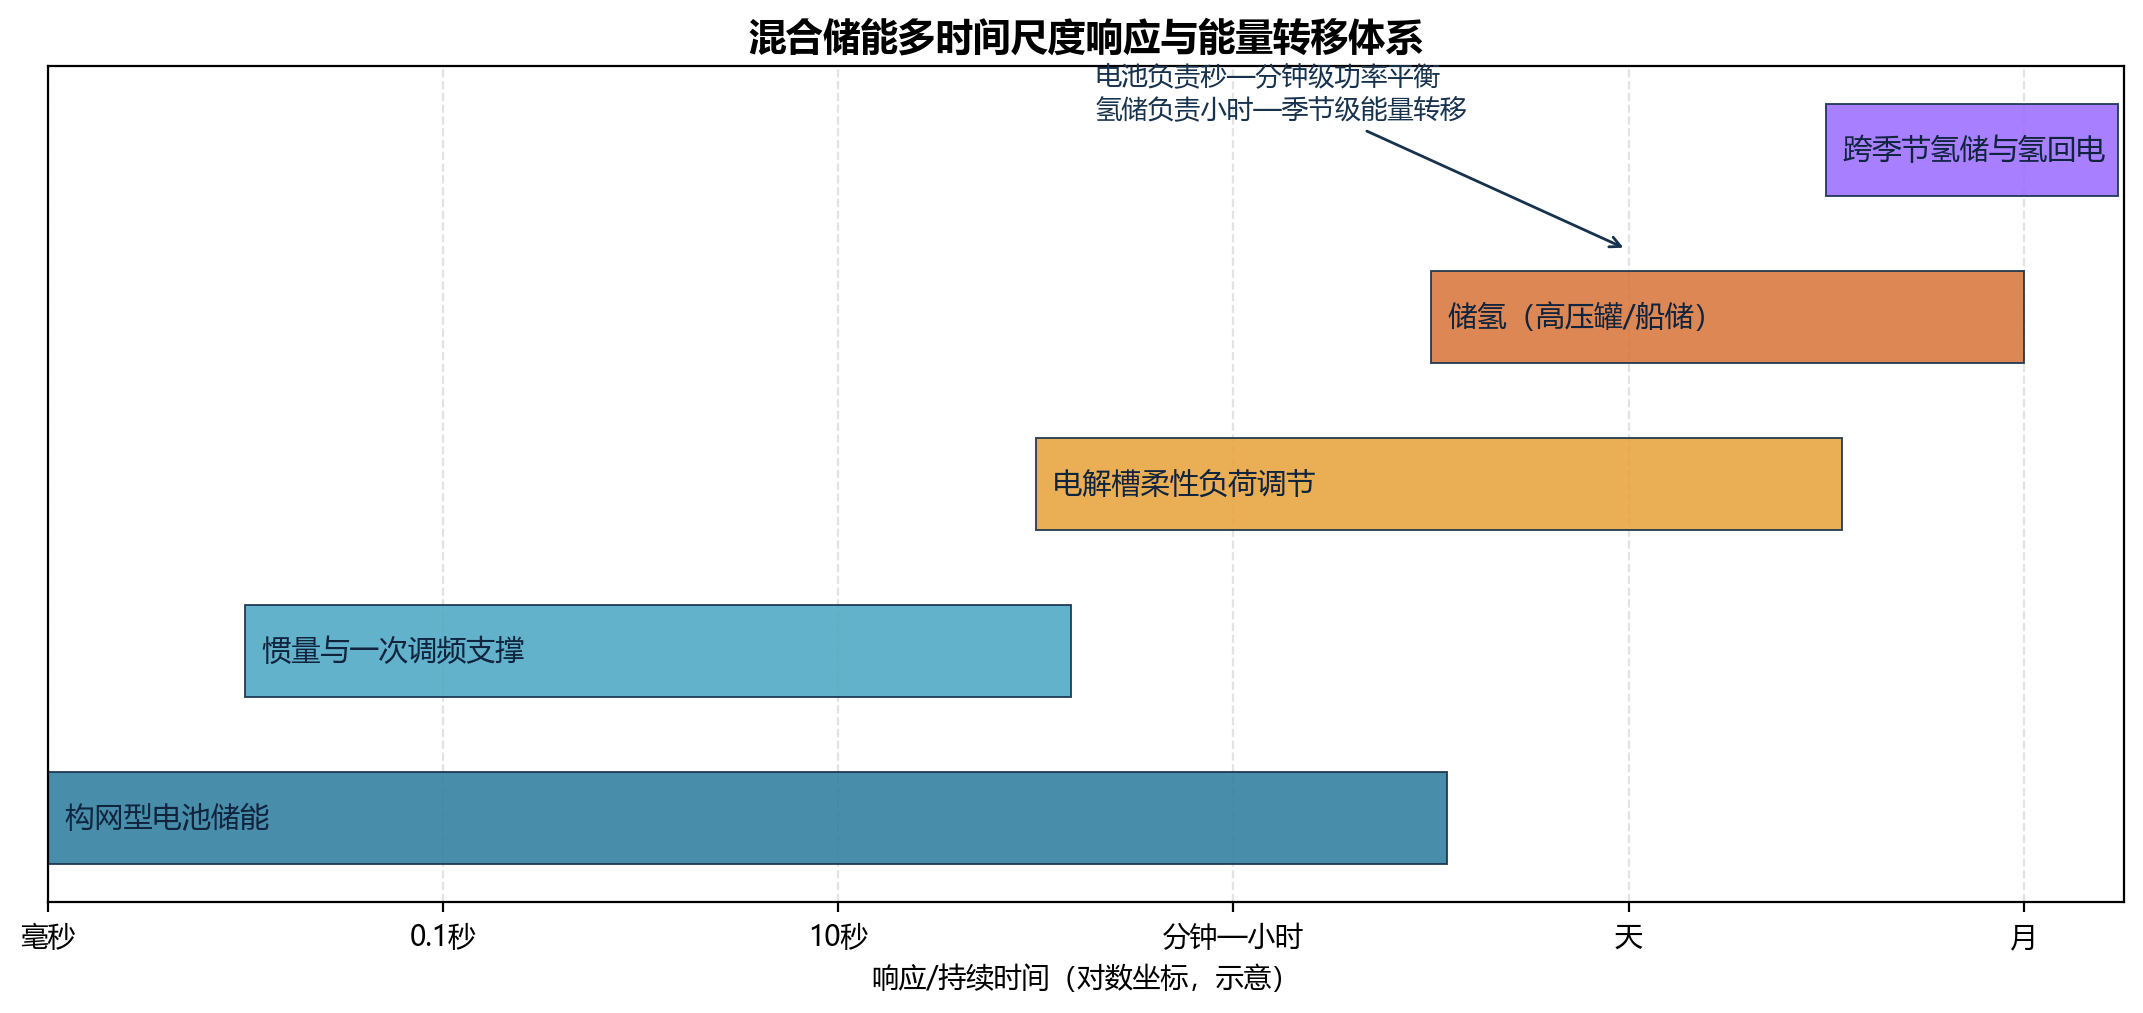
\includegraphics[width=0.98\textwidth]{figures/chapter3/fig3-4_storage_timescales.png}
\caption{混合储能的多时间尺度响应与能量转移分工}
\label{fig:c3-storage-timescale}
\sourcetype{项目内部归纳。持续时间边界为示意，不作为设备性能保证。}
\end{figure}

\begin{table}[H]
\centering
\caption{稳定控制、能量调度与长期价值转化的分层责任}
\label{tab:c3-storage-responsibility}
\begin{tabularx}{\textwidth}{p{2.6cm} p{3cm} X X}
\toprule
{\bfseries 层级} & {\bfseries 主要资源} & {\bfseries 核心责任} & {\bfseries 验证方式}\\
\midrule
设备安全层 & PCS、电池管理、电解槽保护、氢安全联锁 & 电流、电压、温度、压力、气体与故障保护 & 型式试验、设备联调、HAZOP/安全审查\\
动态稳定层 & 构网型电池、保护和电源控制器 & 电压频率建立、惯量/下垂响应、限流、故障穿越、黑启动 & 正序动态、EMT、HIL、海试\\
滚动调度层 & 电池、电解槽、算力与外输端口 & 逐时能量分配、SOC/库存、合同与备用约束 & 第4章模型与第5章因果滚动仿真\\
容量规划层 & 电池功率/能量、电解槽、储氢与端口容量 & 在成本、可靠性和价值间选择容量组合 & 第4章容量筛选与第5章敏感性\\
\bottomrule
\end{tabularx}
\sourcetype{项目内部系统分层；构网功能要求参考UNIFI公开规范。}
\end{table}

\subsection{制氢、储氢与可选氢转电链}

制氢链包括水处理、电解、气液分离、纯化、压缩、储存、装卸和安全监测。电解水制氢的
基本能耗、效率和动态模型应以核心期刊综述、设备手册和试验数据为基础
\cite{ursua2012,carmo2013,buttler2018}；第3章只冻结设备链和接口，第4章集中列示公式、
效率、最小负荷、启停、爬坡及库存约束。
\sourcetype{核心期刊论文、制造商公开资料；具体参数须由OEM或企业访谈一手数据确认。}

燃料电池回发不作为本项目主价值链，也不单列独立章节。若场景需要长时保供，可在第4章
制氢—储氢模块中作为可选氢转电支路启用；其容量、效率、最小运行时间和氢耗均应标注为
\assumptiontag，直到取得设备和场景依据。常规方案不得以往返效率较低的氢回电替代
构网电池的快速稳定职责。

\subsection{构网、黑启动与动态校核边界}

构网型资源需要在没有外部强电网参考时形成可控电压和频率，并在电流限制、模式切换、
多机并联及负荷恢复过程中保持稳定。UNIFI规范给出了面向构网型逆变资源的系统级和
设备级功能要求\cite{unifi-v3}，REGFM模型可用于规划层正序动态研究
\cite{regfm-b1}。这些资料不能替代厂家模型，也不能由小时级SOC约束直接推出黑启动
成功。
\sourcetype{国家实验室联盟规范、国家实验室技术报告。}

建议黑启动遵循“构网电池自建母线—关键辅机和通信恢复—电源分级并入—刚性负荷恢复—
柔性负荷分级恢复”的责任链。启动顺序、允许负荷步长、最低SOC和备用时长均需在第5章
动态验证专题或后续HIL中确定；在未完成验证前均为\assumptiontag。

\subsection{储能与制氢接口}

电池向调度层提供SOC、可充/放功率、构网备用占用量、温度和退化状态；电解制氢链提供
可用功率、最小稳定负荷、爬坡、启停状态、氢库存、产品质量和装卸窗口。统一调度只能
使用“扣除安全保留后的可调能力”，不得占用设备控制器为故障和构网支撑保留的裕度。

\section{绿色算力与制氢协同}

\subsection{海底绿色算力的系统角色}

海底算力在本项目中具有双重属性：其一是需要电力、冷却、通信和安全保障的负荷；其二
是通过任务迁移、延迟和功率封顶提供柔性的可计费服务。PUE采用设施总能耗与IT设备能耗
之比的行业定义\cite{green-grid-pue,doe-pue}。项目目标PUE低于1.1为
\assumptiontag，必须明确测量边界、海水温度、泵耗、通信、配电与备用系统是否计入，
并通过实际设计和运行数据验证。
\sourcetype{行业组织资料、政府官网；项目PUE目标待算力运营商和设备商校准。}

算力舱、海缆/光缆、海水换热、备用电源、消防与数据安全应作为一个服务系统设计，不能
仅依据服务器额定功率估算负荷。IT设备更新周期通常短于海工舱体寿命，资产边界和更新
窗口需在第6章单列，具体周期为\assumptiontag。

\subsection{任务分级与柔性边界}

\begin{table}[H]
\centering
\caption{算力任务分级及调度权限}
\label{tab:c3-compute-classes}
\begin{tabularx}{\textwidth}{p{2.5cm} X X X}
\toprule
任务类型 & 典型特征 & 可调动作 & 关键约束\\
\midrule
关键刚性任务 & 连续服务、存储、控制或高SLA业务 & 原则上不参与经济削减 & 供电等级、时延、冗余、备份与恢复\\
可迁移任务 & 可在节点或时间窗口之间转移 & 迁移、错峰、功率封顶 & 截止时间、迁移开销、带宽和数据边界\\
可中断任务 & 批处理、预处理或低优先级任务 & 暂停、重启、降频 & 最大中断时长、重启能耗和进度损失\\
设施辅机 & 冷却、配电、通信、监控与安全系统 & 仅在安全范围内调节 & 环境温度、设备安全和最低连续功率\\
\bottomrule
\end{tabularx}
\sourcetype{项目内部任务分类；任务比例、SLA和调节成本须由算力客户/运营商一手数据校准。}
\end{table}

模型可调的对象是可迁移和可中断任务对应的IT功率，不是全部设施功率。任何削减都应
形成延迟、迁移、服务缺口或违约成本，不能被免费处理。第4章定义状态和约束，第5章
报告有效服务量与违约指标。

\subsection{电—氢—算协同机制}

协同不预设“电优先”“氢优先”或“算力优先”的全年固定排序，而由以下边界共同决定：
\begin{itemize}
  \item 安全优先：构网备用、关键辅机、氢安全和关键算力先满足；
  \item 合同优先：电力计划、氢交付窗口和算力SLA形成必须履约的下限；
  \item 动态可行：电池SOC、电解槽启停和任务迁移限制当前可调范围；
  \item 剩余价值优化：在安全与履约余量内，依据当前价格、预测和机会成本分配剩余功率。
\end{itemize}

提前知道未来48 h或全年真实数据的“完美预见”只可作为理论上界，不得作为实际运行
策略。可部署策略应根据上一时段实测状态、当前可用资源和短期预测滚动更新；具体信息集
与窗口机制由第4章定义。

\subsection{调度大脑的控制层级与降级机制}

调度大脑由设备控制、站级协调和经营优化三层组成。设备控制器拥有保护和紧急停机最高
权限；站级控制维持母线与备用；经营优化在可行域内决定产品分配。通信中断、预测失效、
价格缺失或优化器无解时，系统应退化至经验证的安全规则，包括保留构网容量、满足关键
负荷、限制电解槽与算力爬坡、必要时有序弃能。降级规则本身也是第5章极端场景的测试对象。

\section{多形态输出与海洋综合用能}

\subsection{四类交付端口}

多形态输出不是把所有潜在用途同时建设，而是为不同场址和市场提供可选择、可比较的
标准端口。电力外送、氢能/氨、算力服务和海洋综合用能分别具有独立计量、质量标准、
交付窗口和责任主体。

\begin{table}[H]
\centering
\caption{多形态输出端口及责任边界}
\label{tab:c3-output-ports}
\begin{tabularx}{\textwidth}{p{2.2cm} p{2.3cm} X X}
\toprule
端口 & 交付计量 & 主要工程约束 & 后续责任章节\\
\midrule
电力外送 & 交付点MWh及功率曲线 & 海缆/换流容量、损耗、无功、可用率、并网计划 & 第4章建模；第5章性能；第6章合同\\
氢/氨产品 & 合格氢kg、氨t及批次 & 纯度、压力、库存、装卸窗口、储运与安全 & 第4章氢链；第6章承购和储运\\
算力服务 & 有效设备时、任务量或合同计费单元 & PUE、SLA、时延、带宽、数据和设备更新 & 第4章负荷；第5章服务；第6章合同\\
海洋用能 & MWh或独立服务量 & 淡化、养殖、观测等负荷曲线及作业窗口 & 第4章负荷接口；第6章场景合同\\
\bottomrule
\end{tabularx}
\sourcetype{项目内部接口定义；价格与购买量不在本章设定。}
\end{table}

\subsection{电力、氢氨、算力与海洋服务的边界}

电力端口可根据距离、容量和电网条件选择交流或柔性直流技术，具体损耗和成本函数由
第4章外输模块统一管理，不能用单一“元/公里”跨项目外推。氢能端口以制氢、储氢和
装卸为当前主链，绿氨合成作为预留扩展；若第4章尚无氨合成物料与能量约束，第5章不得
报告绿氨产量或收益。

算力端口只确认完成服务约束的有效任务，不能把全部IT用电直接折算为算力收入。海洋
用能端口需要真实负荷和合同场景；养殖、淡化、观测等空间协同价值若无法独立计量，
只能作为战略或外部性描述，不进入基准现金流。

\subsection{统一计量与数据链}

每个端口至少设置物理计量点、质量/服务计量点和结算计量点。公共母线记录可再生能源
净注入、储能充放、电解与算力用电、外送、辅机和弃能；氢端记录产量、质量、库存和
交付；算力端记录设施功率、IT功率、有效任务和SLA；环境权益由相同时间戳数据生成。
统一数据链是第4章防止能量重复分配、第6章防止收益重复确认的基础。

\section{关键技术、证据归属与成熟度评估}

\subsection{TRL方法与适用边界}

ISO 16290以1至9级定义技术成熟度，虽主要面向空间系统，其分级条件可在明确应用环境后
用于其他领域\cite{iso16290}。本报告据此采用“原理—实验室—相关环境—示范—商业运行”
证据链，但对“深远海、弱网、源储算用一体化”这一新应用环境重新判断。陆上成熟设备
不能因单机TRL高就自动获得深远海系统同等级。
\sourcetype{国际标准｜ISO 16290:2013。}

评估遵循三条规则：一是按本项目使用场景而非一般产品市场评估；二是优先采用政府、
行业协会、上市公司公告、核心期刊和企业访谈一手数据；三是系统成熟度由关键短板约束，
不使用各模块TRL简单平均。当前等级均为项目组基于公开证据的初判\assumptiontag，需由
设备商、检测认证机构和真实海试复核。

\subsection{设备证据的唯一主表}

为消除第1、2、6章的设备资料重复，本报告将设备证据集中登记在表\ref{tab:c3-evidence-home}。
其他章节只引用其结论，不再次展开项目容量、效率、抗台、造价或运行案例。

\begin{table}[H]
\centering
\caption{关键设备证据主归属与参数传递规则}
\label{tab:c3-evidence-home}
\small
\begin{tabularx}{\textwidth}{p{2.5cm} >{\raggedright\arraybackslash}X >{\raggedright\arraybackslash}X}
\toprule
模块 & 本章允许采用的证据 & 向第4章传递的参数类别\\
\midrule
漂浮式风电 & IEC/GB设计要求、认证资料、上市公司公告、OEM曲线、海试与运行数据 & 功率曲线、可用率、切入/切出/复归、辅机与容量边界\\
漂浮式光伏/海洋能 & 行业/国际标准、功率矩阵、型式试验与示范运行数据 & 辐照/海况到功率的映射、停机条件和可用面积\\
构网型电池 & UNIFI等功能规范、厂家模型、型式试验、HIL与现场记录 & SOC、效率、功率/能量、备用占用、爬坡和退化\\
制氢储氢 & 核心期刊、设备手册、试验曲线、产品标准与安全审查 & SEC/效率、最小负荷、启停、爬坡、库存和损耗\\
海底算力 & 行业PUE定义、运营数据、舱体/冷却/通信方案、客户SLA & 刚性/柔性功率、PUE、迁移窗口、服务缺口成本\\
海缆与产品外输 & 设计院方案、供应商报价、工程合同、储运企业和用户访谈 & 容量、损耗、可用率、交付窗口、质量与成本边界\\
\bottomrule
\end{tabularx}

\sourcetype{项目内部证据管理规则。无合同、报价或实测依据的数值均标注为\assumptiontag。}
\end{table}

\subsection{关键技术TRL初判}

\begin{table}[H]
\centering
\caption{蓝海枢纽关键技术TRL初判}
\label{tab:c3-trl}
\footnotesize
\begin{tabularx}{\textwidth}{p{3.5cm} p{1.1cm} X X}
\toprule
技术 & 初判 & 公开证据说明 & 本项目主要缺口\\
\midrule
漂浮式风机组与整机集成 & 8 & 已有示范运行和认证基础 & 大规模场群、长期可靠性与成本\\
漂浮式平台与系泊系统 & 8 & 工程示范及设计规范逐步完善 & 目标海域载荷、疲劳和运维\\
动态海缆与深远海输电 & 8 & 海工与输电已有工程基础 & 超远距离、浮体耦合和维修窗口\\
漂浮式光伏 & 6 & 相关环境示范证据有限 & 深远海耐久、载荷与运维\\
潮流能与波浪能 & 6 & 样机和示范并存 & 经济性、可用率和标准化接口\\
构网型储能（陆上示范） & 7 & 功能规范及现场示范逐步形成 & 深远海平台适配和多机并联\\
深远海平台级离网构网 & 5 & 以模型和局部验证为主 & 真实海况、黑启动、保护与HIL\\
电解水制氢（陆上商业） & 9 & 成熟产品与长期运行经验 & 不代表波动海上环境成熟\\
海上离网制氢与储氢 & 6 & 相关环境示范和方案研究 & 摇摆、盐雾、启停、安全与储运\\
海底绿色算力数据中心 & 9 & 特定场景已有商业运行证据 & 深远海能源岛耦合与长期维护\\
海风直连海底算力 & 8 & 已有工程链路验证 & 弱网运行、任务柔性和规模复制\\
柔性直流/混合直流互联 & 8 & 海上输电已有工程基础 & 本项目容量与距离适配\\
海洋综合用能 & 7 & 风渔等融合链路已有示范 & 独立计量、合同与生态长期评价\\
源储算用协同调度EMS & 6 & 模型、软件和局部功能可验证 & 因果滚动、极端事件和现场闭环\\
\bottomrule
\end{tabularx}
\sourcetype{政府官网、行业协会报告、上市公司公告、核心期刊论文与项目组公开证据研判；所有等级均为\assumptiontag。}
\end{table}

\begin{figure}[H]
\centering
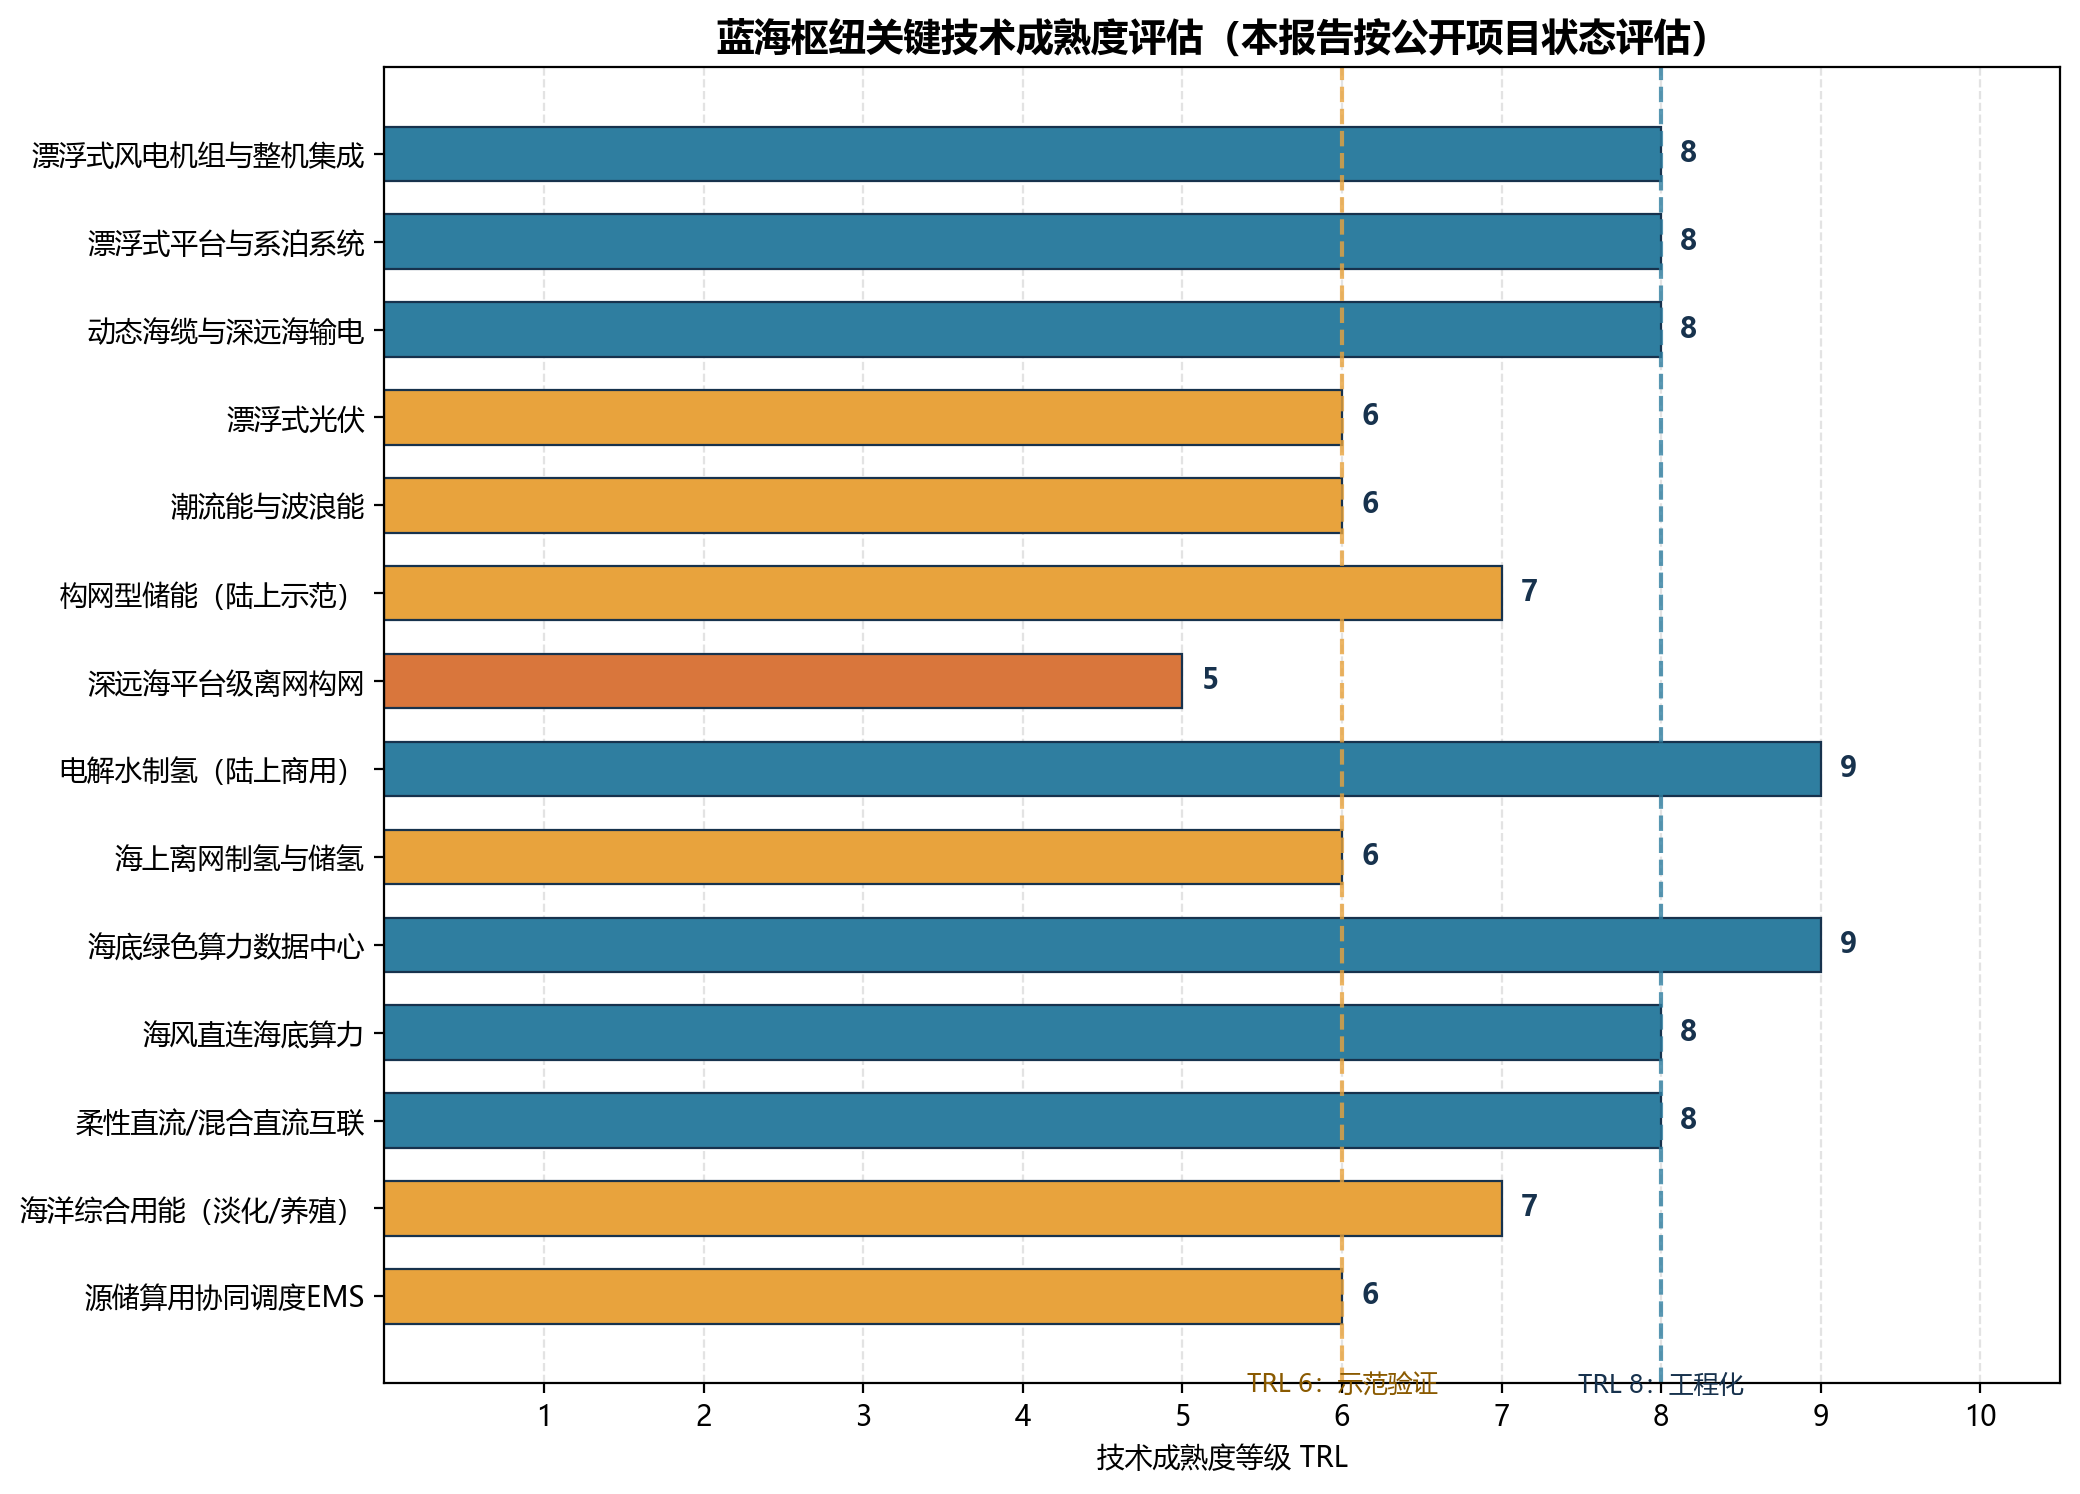
\includegraphics[width=0.98\textwidth]{figures/chapter3/fig3-3_trl_assessment.png}
\caption{蓝海枢纽关键技术TRL初判可视化}
\label{fig:c3-trl}
\sourcetype{项目组依据表\ref{tab:c3-trl}绘制；非认证结论，全部等级待企业和检测机构复核。}
\end{figure}

\subsection{系统短板与优先攻关方向}

从系统集成角度，当前优先级不是继续堆叠高TRL单设备，而是解决四个接口短板：
\begin{enumerate}
  \item 深远海平台级构网、保护、多机并联和黑启动的动态验证；
  \item EMS的因果滚动、预测误差、通信降级与算力SLA联合处理；
  \item 海上波动制氢、储氢、装卸和泄漏处置的一体化安全边界；
  \item 台风等极端事件下的生存停机、关键负荷保障和检查复归流程。
\end{enumerate}

上述短板分别形成第5章测试任务和第6章技术闸门。只有在相关环境验证通过、接口冻结、
性能可写入合同后，单项高成熟技术才可组合为可商业复制的能源枢纽。

\section*{本章小结}
\addcontentsline{toc}{section}{本章小结}

本章完成了源、储、算、用及调度平台的责任分解，明确了物理、数据、控制和计量接口，
并将设备证据与TRL集中为唯一主表。第4章据此只建立可求解模型，第5章只报告场景结果，
第6章只把技术短板转化为投资与示范闸门，从结构上消除了跨章重复。

